\documentclass[12pt,spanish,a4paper]{report}

\usepackage{amssymb}
\setcounter{tocdepth}{3}
\usepackage{url}
\usepackage[utf8x]{inputenc}
\usepackage[spanish]{babel}
\usepackage{graphicx}
\usepackage{hyperref}
\usepackage{listings}
\usepackage{appendix}
\usepackage{makeidx}
\usepackage{fancyhdr}
\usepackage{textcomp}
\usepackage{float}
\usepackage{amssymb, amsmath}
\usepackage{multicol}
\usepackage{anysize}
\usepackage{pdflscape}
\usepackage[usenames,dvipsnames]{color}
\usepackage[font=footnotesize,labelfont=bf]{caption}
\usepackage[T1]{fontenc}  % permite copiar correctamente el texto del pdf.

\hypersetup{
    bookmarks=true,         % show bookmarks bar?
    unicode=false,          % non-Latin characters in Acrobat’s bookmarks
    pdftoolbar=true,        % show Acrobat’s toolbar?
    pdfmenubar=true,        % show Acrobat’s menu?
    pdffitwindow=false,     % window fit to page when opened
    pdfstartview={FitH},    % fits the width of the page to the window
	pdfsubject={Proyecto Final de la carrera Lic. en Ciencias de la Computaci\'on - UNRC},   % subject of the document
    pdftitle={Manual de compilaci\'on e instalaci\'on de FuD-BOINC},    % title
    pdfauthor={Lucas Besso - Ra\'ul Striglio},     % author
    pdfproducer={http://www.fudepan.org.ar/}, % producer of the document
    pdfkeywords={fud} {fud-boinc} {fudepan} {boinc} {tesis} {unrc} {computacion voluntaria} {compilacion} {instalacion} {proyecto} {proyecto boinc}, % list of keywords
    pdfnewwindow=false,      % links in new window
    colorlinks=true,       % false: boxed links; true: colored links
    linkcolor=Red,          % color of internal links
    citecolor=Green,        % color of links to bibliography
    filecolor=Magenta,      % color of file links
    urlcolor=Blue           % color of external links
}

\marginsize{3cm}{3cm}{3cm}{3cm}
\pagestyle{fancy}

\fancyhf{}
\fancyhead[R]{\bfseries\thepage}
\fancyhead[L]{\bfseries\rightmark}

\cfoot{\scriptsize Manual de compilación e instalación de FuD-BOINC }

%Commands
\newcommand{\HRule}{\rule{\linewidth}{0.5mm}}
\renewcommand\lstlistingname{Código}
\renewcommand\lstlistlistingname{Índice de códigos fuente}

\definecolor{gris}{RGB}{245, 245, 245}

%para evitar que corte las palabras
\pretolerance=3000
\tolerance=3000


% Fix the line-breaking
\sloppy


\begin{document}
	\pagenumbering{roman}

	\begin{titlepage} 
		\begin{center}
		
			%Escudos
            \begin{minipage}{0.45\textwidth}
                \begin{center}
                    %Escudo UNRC
                    
\includegraphics[width=60pt,height=90.5pt]{images/escudo.jpg}\\
                    \begin{footnotesize}
                        \textsc{Universidad Nacional de Río Cuarto} \\
                    \end{footnotesize}
                    \vfill
                    \begin{scriptsize}
                        \textsc{Fac. de Cs. Exactas, Fco-Qcas y Naturales} \\
                        \textsc{Departamento de Computación} \\[1cm]    
                    \end{scriptsize}
                \end{center}
            \end{minipage}
            \begin{minipage}{0.45\textwidth}
                \begin{center}
                    %Escudo FuDePAN
                    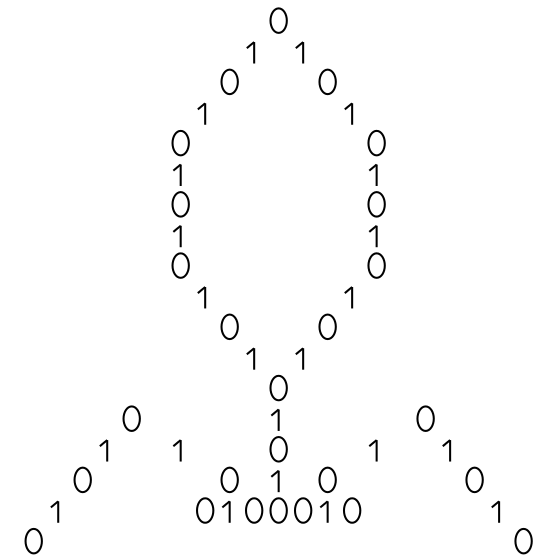
\includegraphics[width=90pt,height=90pt]{images/logo-fudepan.png}\\
                    \vfill
                    \begin{footnotesize}
                        \textsc{FuDePAN} \\
                    \end{footnotesize}
                    \begin{scriptsize}
                        \textsc{Fundación para el Desarrollo de la Programación en Ácidos Nucleicos} \\[1cm]    
                    \end{scriptsize}
                \end{center}
            \end{minipage}

			\textsc{\\[2cm] \large Trabajo Final}\\[0.2cm]
			\textsc{Licenciatura en Ciencias de la Computación}\\[0.2cm]

			\HRule
			{ \Large \bfseries Manual de compilación e instalación de FuD-BOINC\\}
			\HRule 
			\\[4cm]
			

			\begin{multicols}{3}
				\begin{center} \large
					\emph{Autores:}\\
					Lucas \textsc{Besso}\\
					Raúl \textsc{Striglio}
				\end{center}
				\columnbreak  
			
				\begin{center} \large
					\emph{Director:} \\
					Lic. Laura \textsc{Tardivo}
				\end{center}
				\columnbreak  
			
				\begin{center} \large
				\emph{Co-Director:} \\
				Daniel \textsc{Gutson}
				\end{center}
			\end{multicols}
			
			\vfill
			\textit{Última actualización:}
			
			\textit{\today}

		\end{center}
	\end{titlepage}

	\newpage
	
	\tableofcontents
	
	\newpage
	\pagenumbering{arabic}
	
\part{Manual de instalación y compilación de FuD-BOINC}


\chapter{Introducción}

Este documento describe los pasos que se deben seguir para poder compilar la librería FuD con la capa de distribución FuD-BOINC. Para lograr ésto, se explica cómo descargar BOINC, cómo compilarlo y cómo crear un proyecto de computación voluntaria en donde se puedan correr las aplicaciones desarrolladas con FuD-BOINC. Por último, se explican los pasos a seguir para descargar y compilar FuD con las librerías BOINC ya compiladas.

El manual pretende ser un medio simple en donde se integren las pasos necesarios para comenzar a utilizar FuD-BOINC por lo que si se desea extender algunos conceptos y/o instrucciones aquí detalladas recomendamos consultar la información oficial que será incluida con cada sección.



\chapter{BOINC}


\section{Dependencias requeridas}
\label{boinc:dependencias}

Para poder compilar las librerías de BOINC es necesario resolver los requisitos previos del framework.

La información de esta sección está basada de la wiki oficial de BOINC\footnote{\url{http://boinc.berkeley.edu/trac/wiki/ServerIntro\#cookbook-debian40}}.

A continuación se especifican los paquetes necesarios para compilar BOINC basado en sistemas Unix/Linux.

\subsection{Paquetes requeridos por cliente y servidor}

\begin{itemize}
\item m4 
\item make \item autoconf \item automake1.9 \item gcc-4.1 \item gcc \item g++-4.1 \item pkg-config \item libtool \item subversion \item vim
\end{itemize}

\subsection{Paquetes requeridos por el servidor}

\begin{itemize}
\item apache2-mpm-prefork \item libapache2-mod-php5 \item mysql-query-browser \item mysql-client-5.0 \item mysql-server-5.0 \item php5-mysql \item php5-cli \item php5-gd \item phpmyadmin \item python-mysqldb \item libmysql++-dev \item libssl-dev \item openssl
\end{itemize}

\subsubsection{Instalación de Apache}

Para instalar apache y las dependencias para con BOINC\footnote{Para más información consultar: \url{http://www.guia-ubuntu.org/index.php?title=Servidor_web}} instalar los siguientes paquetes:

\begin{itemize}
\item apache2 \item php5 \item libapache2-mod-auth-mysql \item php5-mysql \item phpmyadmin \item libfcgi-dev \item libapache2-mod-fcgid \item php5-cgi \item libcurl3-openssl-dev \item glutg3-dev \item libXmu-dev \item libXi-dev \item libjpeg8-dev
\end{itemize}

\subsection{Paquetes requeridos por el cliente}

\begin{itemize}
\item libssl-dev \item libglut3-dev \item glutg3-dev \item libglui-dev \item libglitz-glx1-dev \item libsdl1.2-dev \item libcurl3-dev \item freeglut3 \item freeglut3-dev \item libsm-dev \item libice-dev \item libxmu-dev \item libxi-dev \item libx11-dev \item libjpeg62-dev \item libgtk2.0-0 \item libgtk2.0-0-dev
\end{itemize}


\section{Configuración de MySQL Server}


Para definir una nueva contraseña del usuario root hacer los siguiente:

\begin{lstlisting}[frame=shadowbox, language=bash, basicstyle=\footnotesize, backgroundcolor=\color{gris}]
mysqladmin -h localhost -u root password mysqlrootpw {or own}
\end{lstlisting}

Para crear un nuevo usuario en la base de datos hacer los siguiente:

\begin{lstlisting}[frame=shadowbox, language=bash, basicstyle=\footnotesize, backgroundcolor=\color{gris}]
mysql -h localhost -u root -p
> GRANT ALL ON *.* TO `boincadm'@`localhost';
> SET PASSWORD FOR `boincadm'@`localhost'=`'; 
\end{lstlisting}

Los permisos deberían ser limitados a la base de datos del proyecto después. Aquí, la definición de una contraseña vacía simplifica el proceso de instalación la cual luego puede ser modificada.


\section{Descarga del código fuente}


El código fuente de BOINC se encuentra almacenado en un repositorio de Subversion (SVN). Correr el siguiente comando para obtener la última versión estable:

\begin{lstlisting}[frame=shadowbox, language=bash, basicstyle=\footnotesize, backgroundcolor=\color{gris}]
svn co http://boinc.berkeley.edu/svn/trunk/boinc
\end{lstlisting}

Para más información consultar la wiki oficial de BOINC\footnote{\url{http://boinc.berkeley.edu/trac/wiki/SourceCode}} que menciona este tema.


\section{Compilación}


Para más información sobre cómo compilar BOINC puede consultar la wiki oficial de BOINC\footnote{\url{http://boinc.berkeley.edu/trac/wiki/BuildSystem}}.

Una vez descargado el código fuente, se puede compilar el software BOINC escribiendo lo siguiente:

\begin{lstlisting}[frame=shadowbox, language=bash, basicstyle=\footnotesize, backgroundcolor=\color{gris}]
./_autosetup
./configure
make
\end{lstlisting}

en el directorio principal, \texttt{boinc/}.

Puede consultar todas las opciones del script \texttt{configure} en la wiki oficial\footnote{\url{http://boinc.berkeley.edu/trac/wiki/BuildSystem\#Configuration}}.


\subsection{Crear un proyecto}
\label{dependencias:crear:proyecto}
Si los que se desea es únicamente crear un proyecto, deberá compilar solamente el servidor:

\begin{lstlisting}[frame=shadowbox, language=bash, basicstyle=\footnotesize, backgroundcolor=\color{gris}]
./configure --disable-client --disable-manager
\end{lstlisting}

\subsection{Compilar el cliente BOINC}

Si lo que se desea es compilar el cliente BOINC para una plataforma específica ejecutar lo siguiente:

\begin{lstlisting}[frame=shadowbox, language=bash, basicstyle=\footnotesize, backgroundcolor=\color{gris}]
./configure --disable-server
\end{lstlisting}

\subsection{Desarrollar aplicaciones BOINC}

Para poder desarrollar aplicaciones BOINC, como en el caso de FuD-BOINC, se debe compilar de la siguiente manera:

\begin{lstlisting}[frame=shadowbox, language=bash, basicstyle=\footnotesize, backgroundcolor=\color{gris}]
./configure --disable-server --disable-client --disable-manager
\end{lstlisting}


\section{Proyecto BOINC}


A continuación se resumen los pasos para la creación de un proyecto BOINC.


\subsection{Dependencias requeridas}

Para poder crear un proyecto es necesario haber compilado el código fuente de BOINC tal como se indica en la sección \ref{dependencias:crear:proyecto}. Para poder efectuar ese paso, es necesario considerar las dependencias mencionadas en la sección \ref{boinc:dependencias}.
			
\subsection{Crear un proyecto}

Toda la información aquí detallada fue tomada de la wiki oficial\footnote{\url{http://boinc.berkeley.edu/trac/wiki/CreateProjectCookbook}}. Consultar allí para más detalles.

Para crear un proyecto BOINC es necesario utilizar la herramienta \texttt{make\_project} proporcionada por BOINC. Para más detalles consultar la wiki oficial que habla sobre esta herramienta\footnote{\url{http://boinc.berkeley.edu/trac/wiki/MakeProject}}.

A partir de la documentación oficial, durante el desarrollo de la tesis FuD-BOINC se ha escrito un simple script que resume los pasos necesarios para que un proyecto quede funcionando. Estos pasos incluyen desde la creación de un proyecto hasta la configuración de permisos de algunos directorios. Dentro del directorio \texttt{Tools/} puede encontrar el script \texttt{createProject} el cual, al ejecutarlo con los parámetros correctos, permite la creación de un proyecto. El script debe ser ejecutado de la siguiente manera:

\begin{lstlisting}[frame=shadowbox, language=bash, basicstyle=\footnotesize, backgroundcolor=\color{gris}]
sudo ./createProject NOMBRE_PROYECTO `DESCRIPCION_PROYECTO'
\end{lstlisting}

y su función es crear un proyecto con el nombre y descripción pasados como parámetros, y de cambiar los permisos de las carpetas para que apache pueda escribir en esos directorios\footnote{\url{http://boinc.berkeley.edu/trac/wiki/ServerIntro/}}.

\textbf{Nota}: \texttt{NOMBRE\_PROYECTO} indica el nombre del proyecto a crear, y \texttt{DESCRIPCION\_PROYECTO} la descripción de dicho proyecto. El proyecto se creará en la ruta: \texttt{~/projects/NOMBRE\_PROYECTO}.


\subsection{Configuración del \texttt{crontab}}

Luego de crear el proyecto, es importante configurar el crontab. Para ello, agregar la siguiente línea con el comando \texttt{crontab -e}:
\begin{lstlisting}[frame=shadowbox, language=bash, basicstyle=\footnotesize, backgroundcolor=\color{gris}]
00,05,10,15,20,25,30,35,40,45,50,55 * * * * ~/projects/NOMBRE\_PROYECTO/bin/start --cron  >/dev/null
\end{lstlisting}


\subsection{Configuración de un proyecto}
\label{project:config}

La configuración de tu proyecto BOINC es controlada por un archivo llamado \texttt{~/projects/NOMBRE\_PROYECTO/config.xml} que es creado por el script \texttt{make\_project}. Es necesario editar este archivo para iniciar un proyecto. 

Se recomienda consultar información detallada sobre cómo configurar este archivo en la wiki oficial de BOINC\footnote{\url{http://boinc.berkeley.edu/trac/wiki/ProjectConfigFile/}}.

\subsection{Agregar aplicaciones al proyecto}
\label{boinc:xadd}
Para agregar las aplicaciones se deben efectuar los siguientes pasos:

\begin{itemize}
\item Editar el archivo de configuración \texttt{config.xml} y eliminar los items relacionados a la aplicación de prueba \texttt{uppercase}.
\item Agregar la aplicación al archivo \texttt{project.xml}.
\item Asegurarse que la base de datos del proyecto esté disponible.
\item Ejecutar los siguientes comandos:

\begin{lstlisting}[frame=shadowbox, language=bash, basicstyle=\footnotesize, backgroundcolor=\color{gris}]
cd ~/projects/NOMBRE\_PROYECTO/
bin/xadd
bin/update_versions
\end{lstlisting}

y seleccionar que si (\texttt{y}) en todos los pasos que se pregunten.
\end{itemize}

\subsubsection{Agregar nuevas versiones de una aplicación}

Para agregar una nueva versión de una aplicación se deben seguir los siguientes pasos:

\begin{itemize}
\item Agregar la aplicación al archivo \texttt{project.xml} y ejecutar \texttt{bin/xadd}.
\item Escribir una aplicación BOINC y compilarla para la plataforma que desees.
\item Copiar el ejecutable a \texttt{~/projects/NOMBRE\_PROYECTO/apps/APPNAME}
\item Instalar la nueva versión ejecutando los mismos comandos mencionados en la sección \ref{boinc:xadd}.
\item Reiniciar el proyecto.
\end{itemize}


\chapter{FuD-BOINC}


\section{Dependencias requeridas}

Para poder compilar la librería FuD-BOINC es necesario resolver los requisitos de la misma.
A continuación se especifican los paquetes necesarios para compilar la librería sobre sistemas Unix/Linux.\\

\subsection{Dependencias de FuD}

\subsubsection{Mili} 
El código fuente de Mili se encuentra alojado en un repositorio de Subversion en googlecode\footnote{\url{http://code.google.com/p/mili/}}. Para descargar la última versión del trunk correr el siguiente comando:

\begin{lstlisting}[frame=shadowbox, language=bash, basicstyle=\footnotesize, backgroundcolor=\color{gris}]
svn checkout http://mili.googlecode.com/svn/trunk/ mili-read-only
\end{lstlisting}

Para conocer los pasos de instalación, consultar el archivo README.

\subsubsection{Boost 1.42 o superior}

Descargar e instalar los paquetes: 

\begin{itemize}
 \item libboost-system 
 \item libboost-thread
\end{itemize}


\subsection{Dependencias de FuD-BOINC}

Descargar e instalar los paquetes:
\begin{itemize}
 \item glibc
 \item libssl-dev
 \item libmysqlclient-dev
\end{itemize}

Se deben tener correctamente instaladas las siguientes librerías de BOINC:

\begin{itemize}
 \item librerías de BOINC
 \item libboinc
 \item libboinc\_api
 \item libsched
 \item libboinc\_crypt
\end{itemize}


\section{Descarga del código fuente}

El código fuente de FuD-BOINC se encuentra almacenado en un repositorio de Subversion (SVN). Correr el siguiente comando para obtener la última versión estable:

\begin{lstlisting}[frame=shadowbox, language=bash, basicstyle=\footnotesize, backgroundcolor=\color{gris}]
 svn checkout https://fud.googlecode.com/svn/branches/boinc FuD-BOINC
\end{lstlisting}

Si bien el código fuente de FuD-BOINC es descargado desde un branch, en un futuro estará disponible en la versión trunk de FuD.

\section{Compilación}

Una vez descargado el código fuente se debe proceder con los siguientes pasos para la compilación e instalación de la librería FuD-BOINC:

\begin{enumerate}
\item Crear un directorio donde se compilará el código fuente.
\item Ingresar al nuevo directorio.
\item Ejecutar el comando:

\begin{lstlisting}[frame=shadowbox, language=bash, basicstyle=\footnotesize, backgroundcolor=\color{gris}]
cmake -Dmiddleware=boinc [options] PATH_TO_Fud-BOINC_Source 
\end{lstlisting}

Debemos destacar que la opción \textbf{-Dmiddleware=boinc} debe ser utilizada para compilar con la capa de distribución implementada con BOINC. Si ésta opción no se la especifica, se compilará con la implementación por defecto(ASIO).

A continuación se destacan las opciones (\texttt{options}) de compilación de FuD-BOINC:

\begin{itemize}
 \item \textbf{-Dboinc\_source=PATH:} utilizar ésta opción para especificar el PATH del directorio de código fuente de BOINC. Por defecto PATH = ``~/boinc''
 \item \textbf{-DCMAKE\_BUILD\_TYPE=Debug:} especificar ésta opción si se desea compilar con el flag para dar soporte a la depuración.
 \item \textbf{-DCMAKE\_COVER\_ON=on:} especifiar ésta opción si se desea compilar con los flags para dar soporte a la cobertura de código.
\end{itemize}
\end{enumerate}


\section{Instalación}

Una vez compilado, solo se debe ejecutar lo siguiente:

\begin{lstlisting}[frame=shadowbox, language=bash, basicstyle=\footnotesize, backgroundcolor=\color{gris}]
sudo make install
\end{lstlisting}


\chapter{Aplicación de prueba Parallel-Clusterer}

Para poder compilar la aplicación Parallel-Clusterer es necesario resolver los requisitos de la misma. A continuación se especifican los paquetes necesarios para compilar la aplicación sobre sistemas Unix/Linux.

\section{Dependencias requeridas}

\subsection{Biopp}

El código fuente de Biopp se encuentra almacenado en un repositorio de Mercurial (hg). Correr el siguiente comando para obtener la última versión estable:

\begin{lstlisting}[frame=shadowbox, language=bash, basicstyle=\footnotesize, backgroundcolor=\color{gris}]
 hg clone https://code.google.com/p/biopp/
\end{lstlisting}

Luego reemplazar el archivo Makefile del directorio descargado por el que se provee en el directorio \texttt{Makefiles/Biopp} del CD.

Para su instalación: ejecutar el comando ``make'' y luego ``make install''.

\subsection{Prot-filer}

El código fuente de Prot-filer se encuentra almacenado en un repositorio de Mercurial (hg). Correr el siguiente comando para obtener la última versión estable:

\begin{lstlisting}[frame=shadowbox, language=bash, basicstyle=\footnotesize, backgroundcolor=\color{gris}]
hg clone https://code.google.com/p/prot-filer/
\end{lstlisting}

Luego reemplazar el archivo Makefile del directorio descargado por el que se provee en el directorio \texttt{Makefiles/Prot-filer}.

Para su instalación: ejecutar el comando ``make'' y luego ``make install''.

\subsection{Getopt\_pp}

El código fuente de Getopt\_pp se encuentra almacenado en un repositorio de Mercurial (hg). Correr el siguiente comando para obtener la última versión estable:

\begin{lstlisting}[frame=shadowbox, language=bash, basicstyle=\footnotesize, backgroundcolor=\color{gris}]
 hg clone https://code.google.com/p/getoptpp/
\end{lstlisting}

Para su instalación: seguir los pasos indicados en el archivo README. Debemos destacar que se deben compilar librerías estáticas.

\subsection{xdrfile}

Descargar la librería desde la siguiente dirección: \url{http://download.fedora.redhat.com/pub/fedora/linux/releases/15/Everything/source/SRPMS/xdrfile-1.1-4.fc15.src.rpm}.

Para su instalación: seguir los pasos indicados en el archivo INSTALL.

\subsection{Feca}

El código fuente de feca se encuentra almacenado en un repositorio de Mercurial (hg). Correr el siguiente comando para obtener la última versión estable:

\begin{lstlisting}[frame=shadowbox, language=bash, basicstyle=\footnotesize, backgroundcolor=\color{gris}]
 hg clone https://code.google.com/p/feca/
\end{lstlisting}

Luego reemplazar el archivo Makefile del directorio descargado por el que se provee en el directorio \texttt{Makefiles/feca}.

Para su instalación: ejecutar el comando ``make'' y luego ``make install''.


\section{Descarga del código fuente}

El código fuente de la aplicación Parallel-clusterer se encuentra almacenado en un repositorio de Subversion (SVN). Correr el siguiente comando para obtener la última versión estable:

\begin{lstlisting}[frame=shadowbox, language=bash, basicstyle=\footnotesize, breaklines=true, backgroundcolor=\color{gris}]
svn checkout http://parallel-clusterer.googlecode.com/svn/branches/biopp parallel-clusterer
\end{lstlisting}

Notar que la descarga se efectúa desde el branch biopp ya que aún no se ha unificado esta versión al trunk.


\section{Compilación}

Para compilar la aplicación, primero se debe reemplazar el archivo ``Makefile'' original por el que se provee en el directorio \texttt{Makefiles/Parallel-Clusterer} perteneciente al CD de éste proyecto. Luego se debe ejecutar el comando ``make'' para compilar la aplicación.

\section{Ejecución}

Para ejecutar la aplicación compilada con FuD-BOINC, primero se debe agregar la aplicación al proyecto BOINC siguiendo los pasos especificados en la sección \ref{boinc:xadd}. Luego, desde el directorio del proyecto, ejecutar el siguiente comando:

\begin{lstlisting}[frame=shadowbox, language=bash, basicstyle=\footnotesize, backgroundcolor=\color{gris}]
bin/clusterer -i [input\_file] -f compressed -s [output\_file] -a full\_cache. 
\end{lstlisting}

Donde:

\begin{itemize}
\item \texttt{input\_file}, es el archivo que se provee en el directorio CD-Tesis/Parallel-clusterer/input\_files/.\\
\item \texttt{output\_file}, es el nombre del archivo de salida donde la aplicación escribirá las estadísticas resultantes.
\end{itemize}


\end{document}